\documentclass{beamer} % Use handout to get rid of repeated slides
\usetheme{AnnArbor}
\usecolortheme{default}
\usefonttheme{professionalfonts}
\usepackage{mathpazo}
\usepackage{listings}
\usepackage{xcolor}

% Define colors
\definecolor{myred}{RGB}{163,0,0}
\definecolor{ttcolor}{RGB}{0,0,1}%{RGB}{163,0,0}
\definecolor{mygray}{RGB}{248,249,250} 
\definecolor{mygreen1}{RGB}{0,96,0}
\definecolor{mygreen2}{RGB}{229,239,229}
\definecolor{aristotelgreen}{HTML}{008A44}
\definecolor{aristotelred}{HTML}{9E0101}
\definecolor{aristotelgrey}{HTML}{2E2E2E}
\definecolor{aristoteldarkred}{HTML}{500101}
\definecolor{aristotelorange}{HTML}{FF8C00}

\setbeamertemplate{theorem}[ams style]
\setbeamertemplate{theorems}[numbered]

\usepackage{etoolbox}

\undef{\definition}
\theoremstyle{definition}
\newtheorem{definition}{\translate{Definition}}
\hypersetup{
	colorlinks=true,
	linkcolor=aristotelorange,   % color for normal internal links
	citecolor=aristotelgreen,   % color for citation links
	urlcolor=aristotelgreen      % color for external links
}

\setbeamercolor{palette primary}{bg=aristotelred, fg=white}
\setbeamercolor{palette secondary}{bg=aristoteldarkred, fg=white}
\setbeamercolor{palette tertiary}{bg=black, fg=white} 

\setbeamercolor{title}{fg=white, bg=aristotelred} % Title text color
\setbeamercolor{subtitle}{fg=white, bg=aristotelred} % Subtitle text color
\setbeamercolor{background canvas}{bg=aristotelgrey} % Background for content canvas
\setbeamercolor{normal text}{fg=white} % Normal text color
\setbeamercolor{titlegraphic}{bg=mygray} % Background color for title graphic area
\setbeamercolor{frametitle}{fg=white, bg=aristoteldarkred}

% Change color of numbered circles in the table of contents
\setbeamercolor{section number projected}{bg=white, fg=black}
\setbeamercolor{subsection number projected}{bg=aristotelred, fg=aristotelgrey}
\setbeamercolor{subsection number projected}{bg=aristotelorange, fg=white}

\setbeamercolor{block title}{fg=white,bg=mygreen1}
\setbeamercolor{block body}{fg=black,bg=mygreen2}


\lstdefinestyle{rstyle}%
{language=[LaTeX]TeX,
	basicstyle=\footnotesize\ttfamily,
	backgroundcolor = \color{mygray},
	commentstyle=\slshape\color{green!50!black},
	keywordstyle=\color{blue},
	identifierstyle=\color{blue},
	stringstyle=\color{orange},
	%escapechar=\#,
	rulecolor = \color{mygray}, 
	showstringspaces = false,
	showtabs = false,
	tabsize = 2,
	emphstyle=\color{red},
	frame = single} 

\begin{document}
	\title[HW: IVs]{Homework}
	\subtitle[subtitle?]{Assigning Instrumental Variables\\
						 Case of Bulgarian Communist Era Wages (1986)}
	\author[Riste Petrov]{Riste Petrov \\ \href{mailto:riste@uni-sofia.bg}{riste@uni-sofia.bg}}
	\institute[AEEM - FEBA]{AEEM - FEBA - Sofia University St. Kliment Ohridski - coh. 2026/27}
	\titlegraphic{\includegraphics[scale=0.5]{/home/anonymous/Documents/Mega/ЦЕЛ/Master/1Courses/SU ENG White horizontal.pdf}}
	\date{\today}
	
	\begin{frame}[fragile]
		\titlepage
	\end{frame}
	
	\begin{frame}[fragile]
		\frametitle{Contents}
		\tableofcontents[]
	\end{frame}
		
	\section{Class Model}
	\begin{frame}[fragile]
		\frametitle{Class Model}
		\framesubtitle{Specification}
		\begin{table}[!htbp]
			\centering
			\begin{tabular}{lrrrr}
				\multicolumn{5}{l}{Dependent Variable: LOG(WAGE)} \\        \multicolumn{5}{l}{Method: Two-Stage Least Squares} \\        \multicolumn{2}{l}{Date: 03/19/26} & \multicolumn{3}{l}{} \\        \multicolumn{2}{l}{Sample: 1 10500 IF WAGE > 0} & \multicolumn{3}{l}{} \\        \multicolumn{2}{l}{Included Observations: 10331} & \multicolumn{3}{l}{} \\        
				\multicolumn{5}{l}{Instrument Specification: C, GRADES, FL, READ, RELIG} \\
			\end{tabular}
		\end{table}
	\end{frame}


	\begin{frame}[fragile]
		\frametitle{Class Model}
		\framesubtitle{Coefficients}
			\begin{table}[!htbp]
				\centering
				\resizebox{\textwidth}{0.85\height}{ % Scale the height to 80% of the current height
				\begin{tabular}{l r r r r}
					\hline
					\multicolumn{1}{c}{Variable} & \multicolumn{1}{r}{Coefficient} & \multicolumn{1}{r}{Std. Error} & \multicolumn{1}{r}{t-Statistic} & \multicolumn{1}{r}{Prob.} \\
					\hline
					\multicolumn{1}{c}{C} & \multicolumn{1}{r}{0.372735} & \multicolumn{1}{r}{0.156603} & \multicolumn{1}{r}{2.380133} & \multicolumn{1}{r}{0.0173} \\
					\multicolumn{1}{c}{EDU} & \multicolumn{1}{r}{-0.033558} & \multicolumn{1}{r}{0.023950} & \multicolumn{1}{r}{-1.401175} & \multicolumn{1}{r}{0.1612} \\
					\multicolumn{1}{c}{INNOV} & \multicolumn{1}{r}{0.011635} & \multicolumn{1}{r}{0.022960} & \multicolumn{1}{r}{0.506721} & \multicolumn{1}{r}{0.6124} \\
					\multicolumn{1}{c}{MAJOR} & \multicolumn{1}{r}{0.530028} & \multicolumn{1}{r}{0.020033} & \multicolumn{1}{r}{26.45774} & \multicolumn{1}{r}{0.0000} \\
					\multicolumn{1}{c}{MALE} & \multicolumn{1}{r}{0.238713} & \multicolumn{1}{r}{0.019011} & \multicolumn{1}{r}{12.55664} & \multicolumn{1}{r}{0.0000} \\
					\multicolumn{1}{c}{BKP} & \multicolumn{1}{r}{0.404941} & \multicolumn{1}{r}{0.197271} & \multicolumn{1}{r}{2.052710} & \multicolumn{1}{r}{0.0401} \\
					\multicolumn{1}{c}{AGE} & \multicolumn{1}{r}{0.099950} & \multicolumn{1}{r}{0.003029} & \multicolumn{1}{r}{32.99719} & \multicolumn{1}{r}{0.0000} \\
					\multicolumn{1}{c}{AGE\textasciicircum 2} & \multicolumn{1}{r}{-0.001028} & \multicolumn{1}{r}{2.69E-05} & \multicolumn{1}{r}{-38.18487} & \multicolumn{1}{r}{0.0000} \\
					\hline
					\multicolumn{1}{l}{R-squared} & \multicolumn{1}{r}{0.307434} & \multicolumn{2}{l}{Mean dependent variable} & \multicolumn{1}{r}{2.667893} \\
					\multicolumn{1}{l}{Adjusted R-squared} & \multicolumn{1}{r}{0.306964} & \multicolumn{2}{l}{S.D. dependent var} & \multicolumn{1}{r}{0.829038} \\
					\multicolumn{1}{l}{S.E. of regression} & \multicolumn{1}{r}{0.690164} & \multicolumn{2}{l}{Sum squared residuals} & \multicolumn{1}{r}{4917.112} \\
					\multicolumn{1}{l}{F-statistic} & \multicolumn{1}{r}{696.8929} & \multicolumn{2}{l}{Durbin-Watson statistic} & \multicolumn{1}{r}{1.959189} \\
					\multicolumn{1}{l}{Prob(F-statistic)} & \multicolumn{1}{r}{0.000000} & \multicolumn{2}{l}{Second-Stage SSR} & \multicolumn{1}{r}{4776.209} \\
					\multicolumn{1}{l}{J-statistic} & \multicolumn{1}{r}{147.8605} & \multicolumn{2}{l}{Instrument rank} & \multicolumn{1}{r}{10} \\
					\multicolumn{1}{l}{Prob(J-statistic)} & \multicolumn{1}{r}{0.000000} & \multicolumn{1}{c}{} & \multicolumn{1}{c}{} & \multicolumn{1}{c}{} \\
					\hline \\ [-4.5pt]
				\end{tabular}
				}
			\end{table}
	\end{frame}
	
	\begin{frame}[fragile]
		\frametitle{Class Model}
		\framesubtitle{Exogeneity Test}
		\begin{center}
		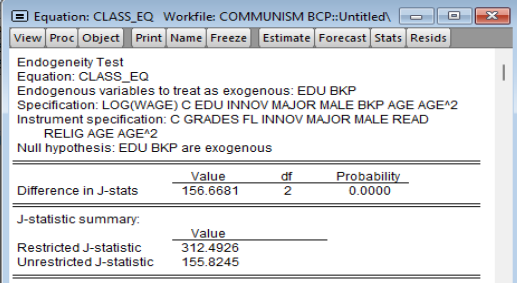
\includegraphics[width=0.9\textwidth]{exogeneity.png}
		\end{center}
	\end{frame}
	
	
	
	\begin{frame}[fragile]
		\frametitle{Class Model}
		\framesubtitle{Stock Yogo}
		\begin{center}
			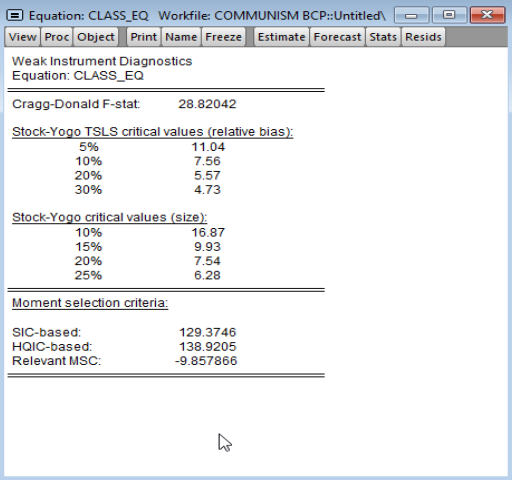
\includegraphics[width=0.6\textwidth]{class_stock_yogo.png}
		\end{center}
		
	\end{frame}
	
	\section{Best Model}
	\begin{frame}[fragile]
		\frametitle{Best Model}
		\framesubtitle{Specification}
		\begin{table}[!htbp]
			\centering
			\begin{tabular}{lrrrr}
				\multicolumn{5}{l}{Dependent Variable: LOG(WAGE)} \\        \multicolumn{5}{l}{Method: Two-Stage Least Squares} \\        \multicolumn{2}{l}{Date: 03/19/26} & \multicolumn{3}{l}{} \\        \multicolumn{2}{l}{Sample: 1 10500 IF WAGE > 0} & \multicolumn{3}{l}{} \\        \multicolumn{2}{l}{Included Observations: 10331} & \multicolumn{3}{l}{} \\        
				\multicolumn{5}{l}{Instrument Specification: C, GRADES, $\text{GRADES}^2$ FL, $\text{FL}^2$} \\
				\multicolumn{5}{l}{INNOV, $\text{INNOV}^2$, RELIG}
			\end{tabular}
		\end{table}
	\end{frame}
	
	
	\begin{frame}[fragile]
		\frametitle{Best Model}
		\framesubtitle{Coefficients}
		\begin{table}[!htbp]
			\centering
			\resizebox{\textwidth}{0.85\height}{ % Allow resizing of the table to fit within text width
				\begin{tabular}{lrrrr}
					\hline
					\multicolumn{1}{c}{Variable} & \multicolumn{1}{r}{Coefficient} & \multicolumn{1}{r}{Std. Error} & \multicolumn{1}{r}{t-Statistic} & \multicolumn{1}{r}{Prob.} \\
					\hline
					\multicolumn{1}{c}{C} & \multicolumn{1}{r}{-0.750072} & \multicolumn{1}{r}{0.143508} & \multicolumn{1}{r}{-5.226673} & \multicolumn{1}{r}{0.0000} \\
					\multicolumn{1}{c}{EDU} & \multicolumn{1}{r}{0.667379} & \multicolumn{1}{r}{0.068620} & \multicolumn{1}{r}{9.725742} & \multicolumn{1}{r}{0.0000} \\
					\multicolumn{1}{c}{EDU\textasciicircum 2} & \multicolumn{1}{r}{-0.103346} & \multicolumn{1}{r}{0.009839} & \multicolumn{1}{r}{-10.50400} & \multicolumn{1}{r}{0.0000} \\
					\multicolumn{1}{c}{AGE} & \multicolumn{1}{r}{0.098050} & \multicolumn{1}{r}{0.002982} & \multicolumn{1}{r}{32.88007} & \multicolumn{1}{r}{0.0000} \\
					\multicolumn{1}{c}{AGE\textasciicircum 2} & \multicolumn{1}{r}{-0.000998} & \multicolumn{1}{r}{2.77E-05} & \multicolumn{1}{r}{-35.99323} & \multicolumn{1}{r}{0.0000} \\
					\multicolumn{1}{c}{BKP} & \multicolumn{1}{r}{0.448531} & \multicolumn{1}{r}{0.170358} & \multicolumn{1}{r}{2.632866} & \multicolumn{1}{r}{0.0085} \\
					\multicolumn{1}{c}{MAJOR} & \multicolumn{1}{r}{0.725095} & \multicolumn{1}{r}{0.026382} & \multicolumn{1}{r}{27.48472} & \multicolumn{1}{r}{0.0000} \\
					\multicolumn{1}{c}{MALE} & \multicolumn{1}{r}{0.183775} & \multicolumn{1}{r}{0.020093} & \multicolumn{1}{r}{9.146081} & \multicolumn{1}{r}{0.0000} \\
					\multicolumn{1}{c}{READ} & \multicolumn{1}{r}{0.148789} & \multicolumn{1}{r}{0.029493} & \multicolumn{1}{r}{5.044949} & \multicolumn{1}{r}{0.0000} \\
					\hline
					\multicolumn{1}{l}{R-squared} & \multicolumn{1}{r}{0.236575} & \multicolumn{2}{l}{Mean dependent var} & \multicolumn{1}{r}{2.667893} \\
					\multicolumn{1}{l}{Adjusted R-squared} & \multicolumn{1}{r}{0.235983} & \multicolumn{2}{l}{S.D. dependent var} & \multicolumn{1}{r}{0.829038} \\
					\multicolumn{1}{l}{S.E. of regression} & \multicolumn{1}{r}{0.724646} & \multicolumn{2}{l}{Sum squared resid} & \multicolumn{1}{r}{5420.201} \\
					\multicolumn{1}{l}{F-statistic} & \multicolumn{1}{r}{574.4696} & \multicolumn{2}{l}{Durbin-Watson stat} & \multicolumn{1}{r}{1.953576} \\
					\multicolumn{1}{l}{Prob(F-statistic)} & \multicolumn{1}{r}{0.000000} & \multicolumn{2}{l}{Second-Stage SSR} & \multicolumn{1}{r}{4686.561} \\
					\multicolumn{1}{l}{J-statistic} & \multicolumn{1}{r}{38.03247} & \multicolumn{2}{l}{Instrument rank} & \multicolumn{1}{r}{13} \\
					\multicolumn{1}{l}{Prob(J-statistic)} & \multicolumn{1}{r}{0.000000} & \multicolumn{1}{c}{} & \multicolumn{1}{c}{} & \multicolumn{1}{c}{} \\
					\hline
				\end{tabular}
			}
			\caption{Regression Results for LOG(WAGE) Using Two-Stage Least Squares}
			\label{tab:log_wage_regression}
		\end{table}
		
	\end{frame}
	
	\begin{frame}[fragile]
		\frametitle{Best Model}
		\framesubtitle{Exogeneity Test}
		\begin{center}
			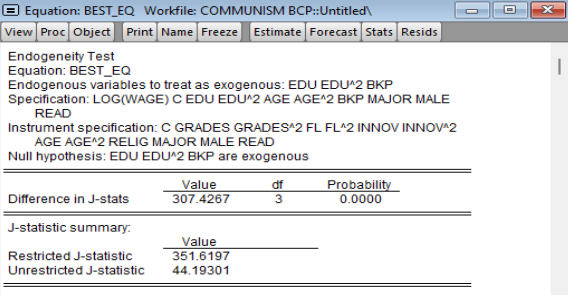
\includegraphics[width=0.9\textwidth]{exog_best.png}
		\end{center}
		
	\end{frame}
	
	
	
	\begin{frame}[fragile]
		\frametitle{Best Model}
		\framesubtitle{Stock Yogo}
		\begin{center}
			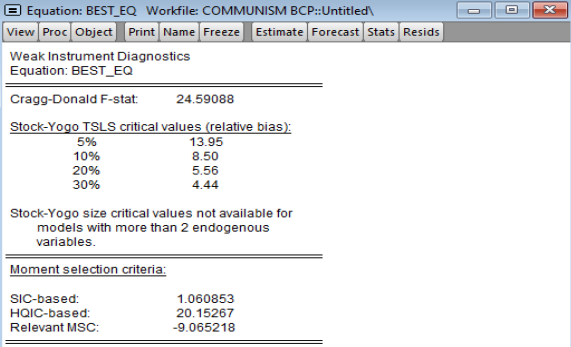
\includegraphics[width=0.9\textwidth]{stock_yogo_best.png}
		\end{center}
	\end{frame}
	
	
	
	
	
	\section{Q\&A}
	\begin{frame}[fragile]
		\frametitle{Ending remarks}
		\begin{center}
			I am delighted for your attention.\\
			\vspace{1em}
			Q \& A?
		\end{center}
	\end{frame}
	
\end{document}